
% C.H. Re-write of this section!

\begin{summary}
Co-I Hirata is leading the development of the HLS observing plan, extending his
previous tools used for the SDT. These tools incorporate observing constraints
in the chosen orbit, an exposure-by-exposure observing sequence optimized with
detailed model of overheads, and tiling/coverage maps including field
distortions and curved sky effects. These tools treat both imaging and
spectroscopy with unified functions and scripts, and are well suited to joint
survey optimization when both hardware parameters (e.g., reaction wheel
orientations) and the observing program (e.g., depth vs.\ area) are considered.
This effort is coordinated with the scheduling and Design Reference Mission (DRM)
Working Groups. We are both providing an example detailed plan for the HLS to
the DRM working group, and cross-checking the Project's spreadsheet-level survey
calculators against our simulations. The HLS observing plan is also being
transferred to the Calibration Working Group, since the HLS observing strategy
feeds directly into the issue of self-calibration.
\end{summary}

\subsection{Survey Optimization Principles}
%==========================================
%\Auth{David W, Chris, Olivier}
\label{sec:sur_opt}

%%%%The key constraint in survey optimization is the limited amount of observational time
%%%%available, since WFIRST is life-time limited and has multiple science focus areas.
%%%%For fixed instrumental capabilities and observing time, the most basic
%%%%decision to make about survey strategy is the trade between depth and total area.
%%%%In optimizing the WFIRST WL and BAO/RSD surveys, there are two key considerations:
%%%%(i) {\em precision} -- to maximize the DE science return of WFIRST, taking advantage of synergy with other surveys; and
%%%%(ii) {\em accuracy} -- tight control of systematic uncertainties, to ensure correct DE measurements.
The key constraint in survey optimization is the limited amount of observational time
available, since WFIRST is life-time limited and has multiple science focus areas.
For fixed instrumental capabilities and observing time, the primary
decisions on survey strategy are the trade between depth and total area, and
the balance between imaging and spectroscopy.
These decisions are driven by two major considerations:
\begin{itemize}
\item \emph{Pecision} -- to maximize the DE science return of WFIRST, taking advantage of synergies with other surveys; and
\item \emph{Accuracy} -- tight control of systematic uncertainties, to ensure correct DE measurements.
\end{itemize}
The combined expertise of our team in WL and GRS enables us to rapidly evaluate
these trades.

\paragraph{HLIS} The statistical power of a WL survey scales with the
total number of galaxy shape measurements, the product of the survey area and the effective surface density.
The SDT2015 report adopts an HLS imaging exposure time that yields roughly equal
contributions from read noise and sky noise in the most sensitive
filters, which approximately maximizes the total number of shape
measurements. This is a compromise between minimizing overheads and
read noise (which favors a ``deep'' mode), versus the shallow number
counts of resolved WL sources (shallower than $N\propto F^{-2}$, which
favors a ``wide'' mode). We re-examined the depth vs.\ area trade using
higher-fidelity tools (e.g., incorporation of shape measurement noise from realistic simulations, and updated
detector properties) and propagating the trades all the way to cosmological parameters
(using \CoLi).

\paragraph{HLSS} The depth vs.\ area trade for the GRS is driven by two
competing factors: for deep surveys, where the number density of galaxies $n$ is
large ($nP\gg 1$, where $P$ is the power spectrum at a given scale), the
information per unit area saturates; whereas for wide surveys, overheads reduce
inefficiency and galaxy shot noise inflates the statistical errors. In the SDT15
survey design, the GRS covers the same area as the HLS imaging survey ($\approx
2,200\deg^2$), to a $7\sigma$ limiting line flux of $\sim 10^{-16}
\erg\cm^{-2}\,{\rm s}^{-1}$ over most of the grism bandpass. This yields
approximately the largest number of galaxy redshifts for a fixed total observing
time. SDT15 found that doubling the survey area at fixed observing time (even
without additional imaging) {\it reduces} the precision of BAO measurements
because of the rapid increase in galaxy shot noise with decreasing spectroscopic
depth. However, this conclusion is sensitive to the luminosity function of
H$\alpha$ emitters at $z=1-2$, which remains uncertain
\cite{Mehta:2015,Pozzetti:2016}; Co-Is Teplitz and Wang lead our efforts to
reduce this uncertainty and feed the results into optimization of the GRS
(\S~\ref{sec:LF}).


\subsection{Snapshot of the HLS observing plan}
\label{ss:snapshot}

\begin{summaryii}
Our team provided a ``snapshot'' of the HLS observing sequence to the full FSWG
on April 19, 2017. This is by no means a final or even optimized version of the
HLS, but is a work in progress as a result of trades in Phase A, as well as the
recent decision to reduce the primary mission to 5 years.
\end{summaryii}

Major updates relative to the SDT plan have included:
\begin{itemize}
\item A Lissajous orbit around L2. This is presently a place-holder, as the exact orbit has not yet been selected (and would depend on the launch date), but it gives a possible sampling of Sun, Earth, and Moon constraints.
\item A rotated WFI (by 90$^\circ$ relative to the Cycle 6 design).
\item Recommended slew and settle times provided by the Project.
\item Faster detector readout (200 kHz instead of 100 kHz).
\item Changes to the exposure time and dithering strategy to accommodate a
5-year baseline mission (as is to be presented to the WIETR). Specifically, we
reduced exposure time to 140.2 s (imaging) and 297.0 s (spectroscopy); and
changed the dither pattern in J band. (We are working on checking this strategy
with image simulations, if it causes a problem we may have to revert.)
\item Implemented bright star avoidance (observations are skipped if there is an $H_{\rm AB}\le 3$ star within 6 arcmin of any SCA).
\end{itemize}
Known current issues with the snapshot plan include:
\begin{itemize}
\item
The SN and coronagraph programs in the code haven't been updated since the SDT
(except to cut the mission time by a factor of 5/6), even though they will
likely change significantly. As in the SDT report, the coronagraph has blocks of
time reserved. This will evolve in order to align the HLS plan with the other
groups, as well as any changes to the scheduling architecture that we are
directed to implement (e.g.\ block scheduling).
\item
We have begun putting the deep fields into this document, but right now they are
(i) not fully specified, (ii) the tiling is not optimized, and (iii) some roll
angles don't align with WFIRST constraints (hence didn't schedule). These issues
will be solved in the next snapshot.
\end{itemize}

We note that \emph{no policy decisions should be inferred from this sequence},
as these will come from a higher level.

The survey bounding box is 2,097 deg$^2$. The area covered with $\ge 3$ exposures
in every filter and the grism, including edge effects and holes around the
bright stars, is 1,947 deg$^2$. The time required for this version of the HLS is
394 days (imaging) + 215 days (spectroscopy).

The scheduling tools output a set of charts, included in this package:
\begin{itemize}
\item
Fig.~\ref{fig:observing_chart}: Graphical display of the 5-year observing sequence.
\item
Fig.~\ref{fig:hls_depth}: HLS distribution of number of exposures in each filter.
\item
Fig.~\ref{fig:hls_dust}: HLS distribution of dust column [$E(B-V)$ in magnitudes]. Cosmological forecasts are based on a dust column of $E(B-V)=0.035$ mag.
\item
Fig.~\ref{fig:hls_bright}: HLS distribution of zodiacal light (normalized to 1 at the ecliptic poles averaged over the year). Cosmological forecasts are based on a zodiacal brightness of 1.60 (except for 1.75 in the F184 filter, which is the least sensitive to zodiacal light and therefore was scheduled at inferior times of year).
\item
Fig.~\ref{fig:footprint}: The footprint of the HLS on the sky. This is an area of ongoing optimization, as we consider the needs of the deep fields, overlap with LSST, and the fraction of the survey footprint accessible from Northern observatories such as Subaru.
\end{itemize}

\begin{figure}
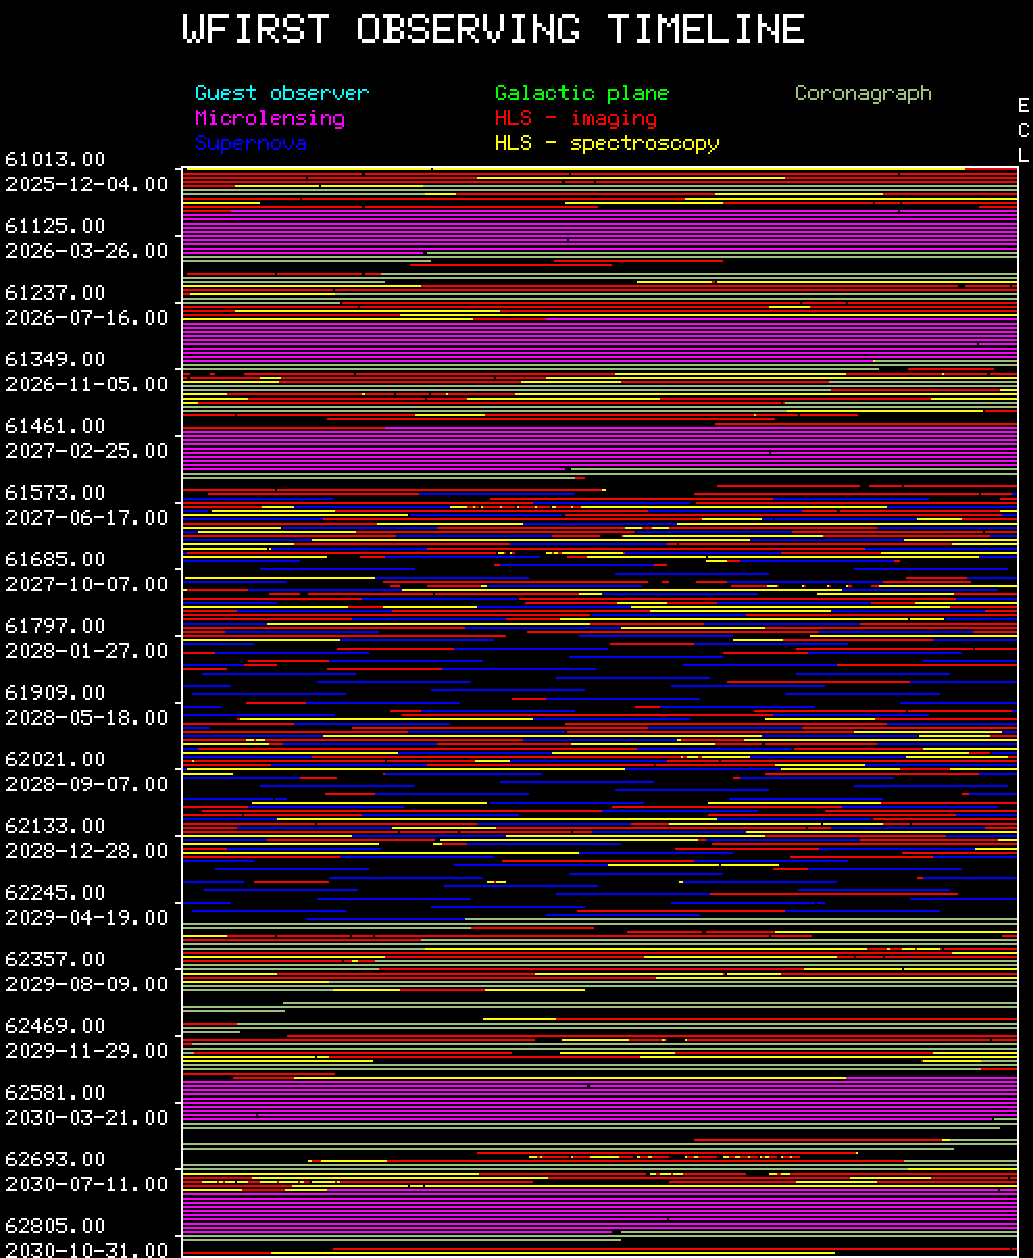
\includegraphics[height=8in]{Plots/observing_chart.pdf}
\caption{\label{fig:observing_chart}Observing timeline. Each row represents 7 days of observations, and is color-coded according to the observing program. Note the microlensing seasons (magenta), supernova survey (blue: $\sim$5-day cadence), and HLS (red+yellow). Blank areas are not allocated. Labels on the left-hand side are shown every 16 weeks.}
\end{figure}

\begin{figure}
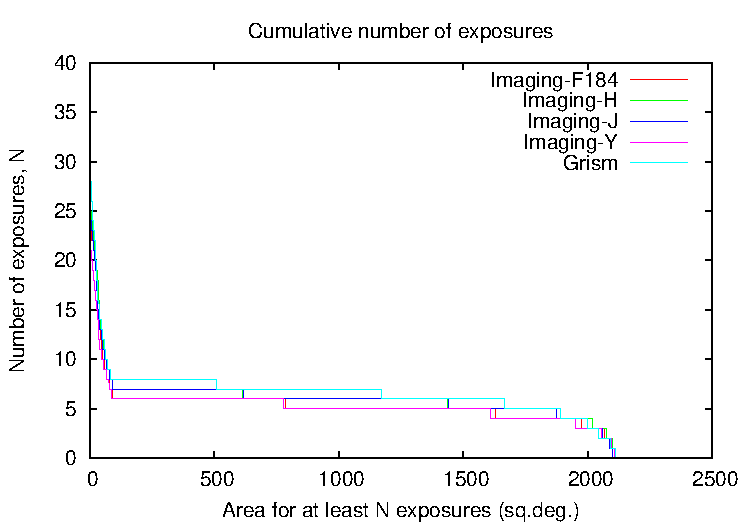
\includegraphics[width=5in]{Plots/hlsdepth.pdf}
\caption{\label{fig:hls_depth}The cumulative distribution of HLS exposure depths above a certain area. The pile-up with many exposures at small area is the result of the deep fields.}
\end{figure}

\begin{figure}
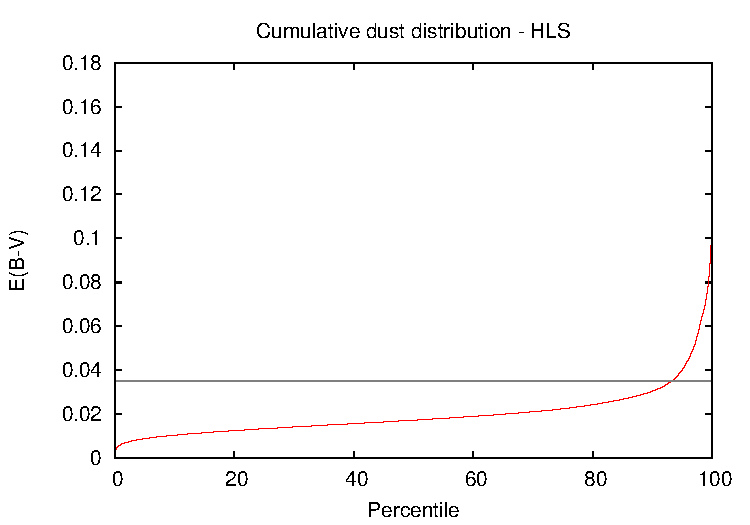
\includegraphics[width=5in]{Plots/hlsdust.pdf}
\caption{\label{fig:hls_dust}The cumulative distribution of Galactic dust in the HLS.}
\end{figure}

\begin{figure}
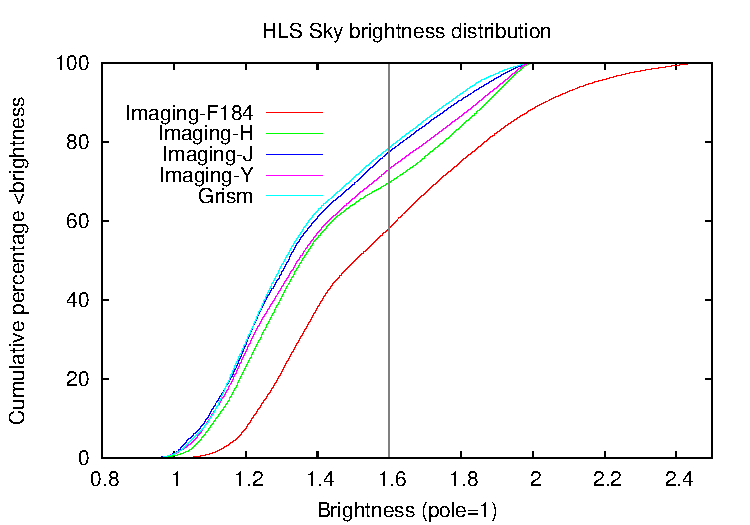
\includegraphics[width=5in]{Plots/hlsbright.pdf}
\caption{\label{fig:hls_bright}The cumulative distribution of zodiacal light in the HLS.}
\end{figure}

\begin{figure}
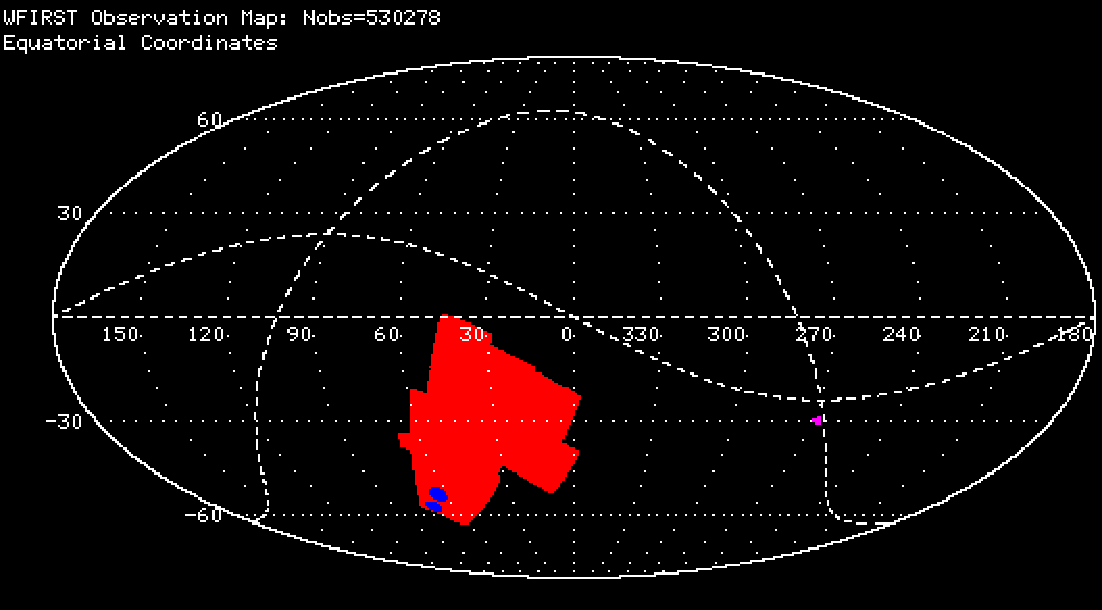
\includegraphics[width=6in]{Plots/sky-equ.pdf}
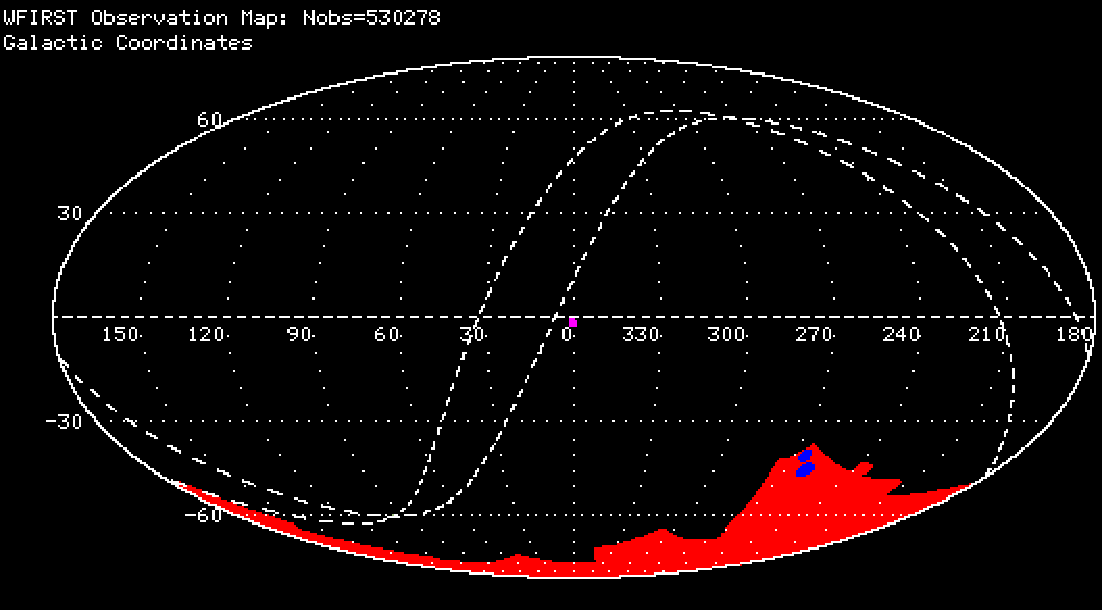
\includegraphics[width=6in]{Plots/sky-gal.pdf}
\caption{\label{fig:footprint}The footprint of the HLS (red) in Equatorial (top) and Galactic (bottom) coordinates.}
\end{figure}

\subsection{Further optimizations}

\begin{summaryii}
Our team plans to study further optimizations to the HLS -- including more
drastic changes such as multi-tiered surveys, or a significant re-balancing of
area vs.\ depth -- in Phase B. However, in preparation for SRR/MDR, our main
focus has been on demonstrating at least one survey configuration that meets
requirements, and the construction of tools that link the observing strategy to
calibration studies (\S\ref{sec:wl_calibration}) and image simulations (\S\ref{sec:hlis_image_sim}).
\end{summaryii}

The optimization of the WFIRST HLS will be tightly linked to operations simulations,
which inform the possible range of footprint area and location, depth in each filter (or grism), redundancy,
and temporal distribution of exposures. We propose a highly integrated approach, with the
operations simulations at the core, but with links to pixel-level simulations to assess required
redundancy, cosmological forecasting tools (\CoLi) to assess science reach, and comparison to the
observing regions of other surveys and telescopes to maximize synergies and meet requirements for
deep fields and photo-$z$ calibration.

% I hope this figure will just be combined with Fig 1.

%
%\setlength\intextsep{-2pt}
%%\begin{center}
%\begin{wrapfigure}{!ht}{0.45\textwidth}
% \begin{boxedminipage}{0.45\textwidth}
% \begin{center}
%\includegraphics[width=1.0\textwidth]{plots/like_DES_WFIRST_combi.eps}
% \end{center}
% \vspace{-1.25cm}
%\caption{{\footnotesize{ \Oli{Initial version for WFIRST vs DES} forecasts multi-probe science case. Probes included are cosmic shear, galaxy clustering, and galaxy-galaxy-lensing from WFIRST (black) in comparison to the Dark Energy Survey (green). The analysis includes BAO, SN1a and Planck information and accounts for galaxy bias, shear calibration, and photo-z errors (with different assumptions for the weak lensing and for the clustering sample). }}}
% \label{tab:milestones}
%\end{boxedminipage}
%\end{wrapfigure}
%% \end{center}
%\setlength\intextsep{0pt}

% \setlength\intextsep{-2pt}
% \begin{wrapfigure}{!ht}{0.75\textwidth}
%  \begin{boxedminipage}{0.75\textwidth}
%  \begin{center}
% \begin{figure*}
% \includegraphics[width=0.5\textwidth]{plots/WFIRST_multi.eps}
%% \caption{\textit{Placeholder plot for WFIRST forecasts multi-probe science case. Probes included are cosmic shear, galaxy clustering, and galaxy-galaxy-lensing, BAO with and without systematics (black and red contours, respectively). The systematics considered in this analysis are shear and photo-z uncertainties (which have different assumptions for the weak lensing and for the clustering sample), and linear galaxy bias. Blue contours include information from DES supernovae type 1a and green contours include an approximate version of Planck CMB temperature and polarization information.}}
%% {\bfseries C.H.: This belongs in another section.}
%%          \label{fi:WFIRST_multi1}
%% \end{figure*}

%\subsection{Synergies of WFIRST internal probes}
%=====================

%\subsection{Synergies of WFIRST and external data sets}
%=====================
